\documentclass[]{aiaa-tc} % insert '[draft]' option to show overfull boxes

 \title{Computing Automatic Analytic Gradients on Sparse Multidisciplinary Design Problems }

\author{
  Tristan A. Hearn,%
     \thanks{Aerospace Engineer, MDAO Branch, Mail Stop 5-10, AIAA Member}
  \ Kenneth T. Moore,%
     \thanks{Senior Systems Engineer, MDAO Branch, Mail Stop 500-105, AIAA Senior Member}
  \ Justin Gray,%
     \thanks{Aerospace Engineer, MDAO Branch, Mail Stop 5-11, AIAA Member}
   \\
  {\normalsize\itshape
  NASA Glenn Research Center, Cleveland, OH}  \\
  John T. Hwang,%
  \thanks{Ph.D. Candidate, Department of Aerospace Engineering, AIAA Student Member}
  \ Joaquim R. R. A. Martins%
  \thanks{Associate Professor, Department of Aerospace Engineering, AIAA Associate Fellow}
  \\
  {\normalsize\itshape
   University of Michigan, Ann Arbor, Michigan, 48109, United States}
}

\AIAAconference{Multidisciplinary Design Optimization Specialist Conference}
\AIAAcopyright{\AIAAcopyrightD{2012}}


% Define commands to assure consistent treatment throughout document
\newcommand{\eqnref}[1]{(\ref{#1})}
\newcommand{\class}[1]{\texttt{#1}}
\newcommand{\package}[1]{\texttt{#1}}
\newcommand{\file}[1]{\texttt{#1}}
\newcommand{\BibTeX}{\textsc{Bib}\TeX}

\setlength{\abovecaptionskip}{0pt}
\setlength{\belowcaptionskip}{0pt}

\usepackage{setspace}

\usepackage{graphicx}
\usepackage{wrapfig}
\usepackage{caption}
\usepackage{amsmath}
\usepackage{lscape}
\usepackage{hyperref}
\usepackage{minted}
\usepackage{color}
\usepackage{appendix}
\usepackage[section]{placeins}

\newcommand{\txt}{\textrm}


\captionsetup[figure]{margin=5pt,font=small,labelfont=bf,textfont=bf,justification=justified,}
%\captionsetup[wrapfigure]{margin=5pt,font=small,labelfont=bf,justification=justified,singlelinecheck=off}
\captionsetup[table]{margin=5pt,font=small,labelfont=bf,textfont=bf,justification=justified,position=top}

\bibliographystyle{aiaa}

\usepackage{lettrine}
\usepackage{verbatim}

\begin{document}

  \maketitle

  \begin{abstract}

  \end{abstract}

  \section{Introduction (Justin)}

    Gradient based optimization with analytic gradients is an effective tool for solving problems 
    with large design spaces. It has been applied widely for aerodynamic shape optimization \cite{Liou2010,palacios2012adjoint}
    and structural optimization\cite{venkataraman2004structural, }. 
    In order to apply these methods to multidisciplinary problems, system level derivatives must be 
    constructed by combining the partial derivatives from each discipline using the Global Sensitivity 
    Equations\cite{Sobieski1990}. This technique has been applied commonly to coupled 
    aero-structural design optimization of aircraft wings\cite{Kenway2012c, Haghighat2012} and is applicable to 
    other coupled design problems such as aero-accoustic design\cite{economon2012coupled}.Extending these 
    gradient based techniques to more complex problem formulations has proved difficult. When 
    design problems grow to include 10's of disciplines, it becomes increasingly difficult to construct the 
    necessary derivatives. Even assuming all of the disciplines could provide analytic partial derivatives, 
    the construction of the system level derivatives is heavily dependent on the structure of the data passing 
    between disciplines. Manual implementations for these problems are time consuming and discourage modifications 
    to the problem formulation in the future. Moore developed a method for automatically assembling the system 
    level derivatives based on the data-dependency graph of a given problem formulation\cite{openmdao_derivatives}. 
    In addition to allowing greater flexibility in the problem formulation, a key feature of this graph-based approach, was the efficient 
    handling of sparse problem formulations. By traversing the graph from design variables to quantities of interest, 
    it was possible to consider only the subset of variables that were relevant to a specific system level gradient thus 
    making gradient computations more efficient. 

    Although Moore's work demonstrated that a framework could compute system level derivatives for arbitrary 
    problem setups, it required components to provide a full Jacobian matrix, which it assembled into 
    complete system level Jacobian matrix.  This made it unsuitable for usage with 
    high-fidelity tools, since they often times had far too many variables to allow assembling a full Jacobian. 
    Martins and Hwang developed an alternative, graph-free, method for computing automatic system 
    level sensitivities which used a global design variable vector\cite{Martins2012}. 
    In a later work they added a matrix-free solver algorithm to their method that solved issue with full Jacobians from 
    Moore's implementation. They demonstrated the effectiveness of their method on a design optimization of a small satellite
    with over 25,000 design variables and over 1 million state variables\cite{CADRE2012}. Despite its success,
    the global-vector based approach required all the variables from the system model be 
    included when solving for system level derivatives. This prevented Martins and Hwang's method 
    from taking advantage of sparsity in the problem formulation and resulted in a less efficient gradient solving step. 
    As a result, over 90\% of the compute during convergence time was spent solving a linear system for the system 
    level derivatives. 

    This work combined the graph-based approach taken by Moore with the matrix-free solution algorithm 
    developed by Martins and Hwang to efficiently compute derivatives for sparse, large-scale engineering 
    design problems. The original small satellite design problem was re-run using the new method and 
    a dramatic increase in efficiency was demonstrated. A second design optimization on a wind turbine was 
    also performed. This problem had a more complex structure with stronger multidisciplinary couplings as well as a
    mixture of analytic and finite difference gradients. 

  \section{Unfied Derivatives Computations (John)}
    Short summary of the unified derivatives method and it's implications for forward or adjoint derivatives. 


  \section{Dependency Graph (Ken/Justin)}

    In Moore's original work on computing derivatives from a dependency graph, he employed 
    a discipline based dependency graph, with a node for each discipline and edges describing 
    dependency between the nodes. He employed path finding algorithms, from the NetworkX library\cite{hagberg-2008-exploring}, 
    to compute the relevant set of disciplines for a given derivative. Although this takes advantage of sparsity at 
    one level, by excluding any disciplines that don't directly contribute, it can't handle a second level of sparsity 
    within the relevant disciplines. Even if a given discipline is relevant, some of its variables may still not be 
    because they don't directly affect the quantities of interest. Pate et. al. proposed an alternative dependency graph 
    structure that addressed this problem\cite{graph_problem2013}. Each discipline and all its inputs and outputs are
    represented by nodes with directed edges between them describing their dependencies on each other.
    Figure \ref{fig:sellar_graph} shows a sample graph for the Sellar Problem \cite{AIAA:sellar}
    given in eqn. \ref{eqn:sellar_formulation}. 

    \begin{align}
        \txt{given} & \ \ y_1 = D_1(x_1,y_2,z_1,z_2) \notag
        \\      & \ \ y_2 = D_2(y_1,z_1,z_2) \notag
        \\\txt{min.} &\ \ F(x_1,y_1,y_2,z_2) \notag
        \\\txt{w.r.t.} & \ \ x_1,y_1,y_2,z_1,z_2 \notag
        \\\txt{s.t.} & \ \ G_1(y_1) \geq 0 \notag
        \\     & \ \ G_2(y_2) \geq 0
        \label{eqn:sellar_formulation}
    \end{align}

    \begin{figure}[!htb]\begin{center}
      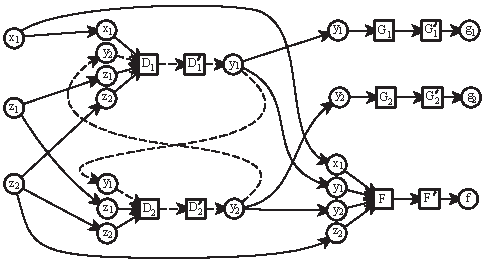
\includegraphics[width=.8\textwidth]{images/sellar_cycles}
      \caption{ Dependency graph for the Sellar problem. \label{fig:sellar_graph}}
    \end{center}\end{figure}

    In the original graph syntax, a single node is given for every variable. This holds true for the graph
    within OpenMDAO, with only one minor caveat. In the case of any hierarchical variables, such as arrays
    or VariableTrees, one variable node is created to represent the overall variable with additional nodes
    created if any specific sub-variable is referenced (e.g., some slice of an array or some child variable from a 
    VariableTree). Figure \ref{fig:subvars} shows how the sub-variable nodes relate to their parent variables. Here,
    both outputs A.x and A.y are array variables. The full array A.x is connected to B.x while a single element
    of A.y is connected to the scalar B.z.

     \begin{figure}[!htb]\begin{center}
      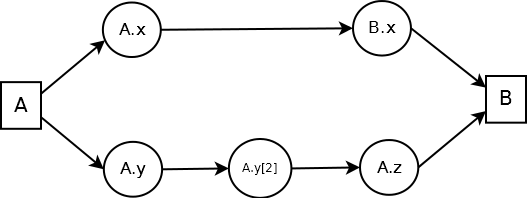
\includegraphics[width=.5\textwidth]{images/Graph1}
      \caption{ Example graph with child nodes for sub-variables \label{fig:subvars}}
    \end{center}\end{figure}

    By representing hierarchical data as a single node, we help keep the overall size of the graph manageable
    when large chunks of data are being communicated. However, if some small sub-set of that data needs to be
    used somewhere it is not correct to indicate a dependence on the entire chunk of data. So in this case, a
    single new node representing the sub-variable is created with its own dependence on the parent variable.
    This book keeping becomes particularly important for when the graph is used to calculate derivatives or
    manage the partitioning of distributed data. Both problems contain large design spaces. The CADRE problem 
    involves about 25000 design variables, and the aero-structural problem involves about 200. 
    Together these problems demonstrate how OpenMDAO can simplify the process of implementing difficult 
    design problems with large design spaces and varying kinds of complexity. 


    \subsection{Determining Execution Order}

    The OpenMDAO framework uses its dependency graph to determine component execution order by finding the 
    shortest path from the design variables to the quantities of interest for any given model\cite{openmdao_derivatives}. 
    This path contains the set of relevant components and variables that make up a sub-graph of the full
    dependency graph. During execution, only the components in this graph will be executed and they will be executed 
    in the order prescribed by following the graph path. 

    \subsection{Cycle Detection and Usage}
    Pate et. al indicate that within a dependency graph, the presence of cycles indicates coupling between
    the components in the cycle \cite{graph_problem2013}. A cycle can consist of two or more components, and
    one component may be part of more than one cycle.

    In formal terms, cycles exist in a graph when a group of nodes are strongly connected. The NetworkX package
    provides an implementation of Tarjans algorithm for finding sets of strongly connected
    components\cite{tarjan1972depth,nuutila1994finding}. Once found, the presence of these cycles
    have an impact on how any given model is solved. Firstly during normal execution, these cycles
    need to be converged with a numerical solver such as Gauss-Seidel or Newton based. 
    In addition these cycles need to be accounted for when solving for the gradients 

    \subsection{Gradient Calculation}
    
    OpenMDAO can calculate a gradient between any set of input and output nodes in the
    dependency graph by setting up the linear system devised by Martins and Hwang \cite{Martins2012} in their 
    work developing a unified theory for derivatives computation. 
    The requested derivatives are calculated from the solution of the set of equations that is assembled
    from the output-input derivatives of all the components. The number of equations 
    is determined by the number of variables represented the graph, which means that the linear 
    system can get very large. To allow for such large systems the full model Jacobian is implemented as 
    a linear operator, so that it never has to be stored entirely in memory. The
    linear operator takes a vector as input, and returns the product of the Jacobian with that vector.
    
    In Martins and Hwang's original work, they considered all possible variables in their linear system. 
    By using the dependency graph, OpenMDAO is able to achieve significant reductions computational cost of 
    solving the linear system. Using the same path finding algorithm for determining execution order, 
    OpenMDAO finds the reduced set of component nodes and variable nodes that are both downstream of the design parameters
    and upstream of a specific quantity of interest. One such sub-graph is found for each linear solve necessary to
    find all the derivatives of the system. It is possible that each sub-graph will contain different sets 
    of variables and components depending on the structure of the graph. Hence, each linear solve step 
    is kept to its minimum possible size to keep. 

    For example, the model in Figure \ref{fig:graph2} contains 5 components that run during an analysis. If we
    want to optimize this model with the given parameter and objective, only the highlighted component nodes
    will be in the reduced dependency graph, and thus only the highlighted variables appear in the linear
    system.
    
    \begin{figure}[!htb]\begin{center}
      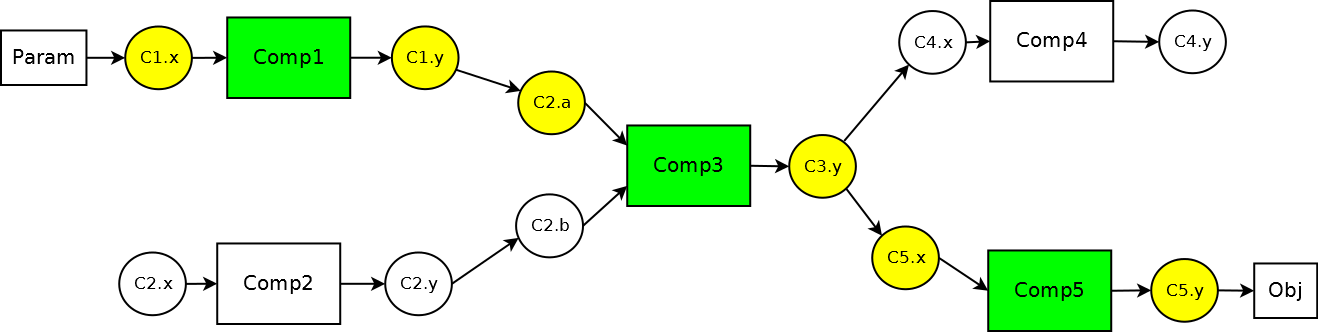
\includegraphics[width=.8\textwidth]{images/Graph2}
      \caption{ The reduced graph for the derivatives calculation includes Comps 1, 3, and 5 with their interconnecting variables. \label{fig:graph2}}
    \end{center}\end{figure}

    \section{Direct vs Adjoint Methods}

    OpenMDAO supports calculating derivatives in two ways: direct and adjoint. The direct method performs
    one linear solve for each design variable. The adjoint method performs one linear solve per each objective 
    and constraints. Hence, if you have more design variables than quantities of interest (as if often the case), 
    the adjoint method will require far fewer solves of the linear system. If you have fewer design variables then 
    objectives and constraints the forward mode is preferable. 

    \subsection{Efficient Handling of Array Variables}
        This graph contains all the necessary information to take full advantage of problem sparsity, 
        but suffers from one potential weakness. A naive implementation of Pate et. al.`s graph would have a 
        single node for each scalar value involved. For a problem with millions of state variables, like 
        aerodynamic shape optimization, the graph would get very large and would be inefficient to operate on. 
        To address this issue related variables, such as arrays, can be aggregated into a single node to
        represent the overall variable. If any specific sub-variable is referenced 
        (e.g., some slice of an array). Figure \ref{fig:subvars} shows how the sub-variable nodes relate to their parent variables. Here,
        both outputs A.x and A.y are array variables. The full array A.x is connected to B.x while a single element
        of A.y is connected to the scalar B.z.

        \begin{figure}[!htb]\begin{center}
          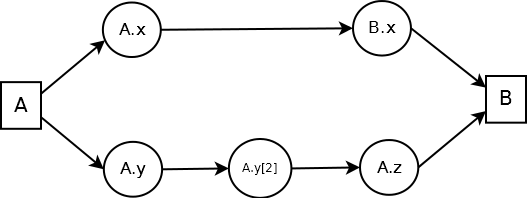
\includegraphics[width=.8\textwidth]{images/Graph1}
          \caption{ Example graph with child nodes for sub-variables \label{fig:subvars}}
        \end{center}\end{figure}

        By using the sub-variable nodes, the computational advantages of problem sparsity are retained. For example, 
        consider $\frac{\partial B.z}{\partial A.y}$ from Fig. \ref{fig:subvars}. Given the graph, we know that
        this derivative will be sparse, with only $A.y[2]$ having non-zero values. When solving for derivatives, 
        without the sub-var node, you would need to consider all the elements of the $A.y$ array. With them, only 
        the single relevant value from the array needs to be considered. 

        \begin{equation} 
            \frac{\partial B.z}{\partial A.y} = 
            \begin{bmatrix} 
                0 \\
                0 \\ 
                \frac{\partial B.z}{\partial A.y[2]} \\
                \vdots \\
                0 \\
            \end{bmatrix}
        \end{equation} 

    \subsection{Graph Traversal and Determining Relevance}

    
        The requested derivatives are calculated from the solution of the set of equations that is assembled
        from the output-input derivatives of all the components. The number of equations
        is determined by the number of variables represented the graph, which means that the linear
        system can get very large. To allow for such large systems the full model Jacobian is implemented as
        a linear operator, so that it never has to be stored entirely in memory. The
        linear operator takes a vector as input, and returns the product of the Jacobian with that vector.

        In Martins and Hwang's original work, they considered all possible variables in their linear system.
        By using the dependency graph, OpenMDAO is able to achieve significant reductions computational cost of
        solving the linear system. Using the same path finding algorithm for determining execution order,
        OpenMDAO finds the reduced set of component nodes and variable nodes that are both downstream of the design parameters
        and upstream of a specific quantity of interest. One such sub-graph is found for each linear solve necessary to
        find all the derivatives of the system. It is possible that each sub-graph will contain different sets
        of variables and components depending on the structure of the graph. Hence, each linear solve step
        is kept to its minimum possible size to keep.

        For example, the model in Figure \ref{fig:graph2} contains 5 components that run during an analysis. If we
        want to optimize this model with the given parameter and objective, only the highlighted component nodes
        will be in the reduced dependency graph, and thus only the highlighted variables appear in the linear
        system.

        \begin{figure}[!htb]\begin{center}
          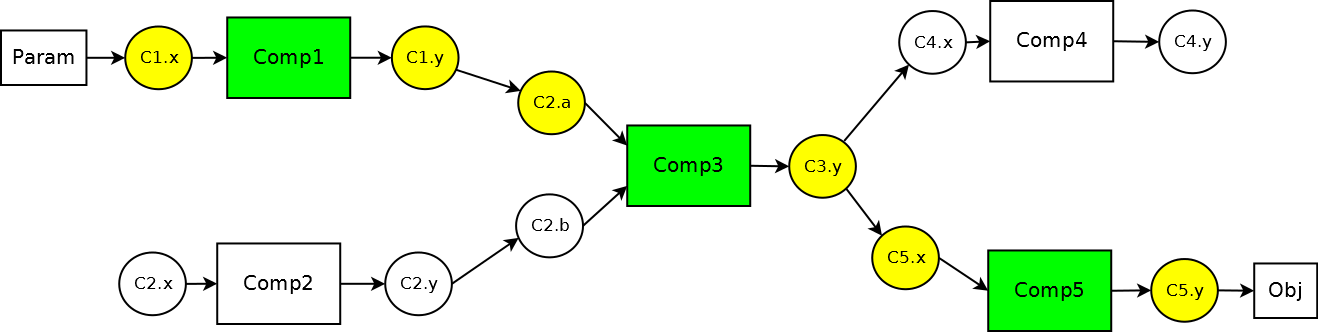
\includegraphics[width=.8\textwidth]{images/Graph2}
          \caption{ The reduced graph for the derivatives calculation includes Comps 1, 3, and 5 with their interconnecting variables. \label{fig:graph2}}
        \end{center}\end{figure}

    
    \subsection{Graph Cycles and Coupled Derivatives}

        Pate et. al indicate that within a dependency graph, the presence of cycles indicates coupling between
        the components in the cycle \cite{graph_problem2013}. A cycle can consist of two or more components, and
        one component may be part of more than one cycle.

        In formal terms, cycles exist in a graph when a group of nodes are strongly connected. The NetworkX package
        provides an implementation of Tarjans algorithm for finding sets of strongly connected
        components\cite{tarjan1972depth,nuutila1994finding}. Once found, the presence of these cycles
        have an impact on how any given model is solved. Firstly during normal execution, these cycles
        need to be converged with a numerical solver such as Gauss-Seidel or Newton based.
        In addition these cycles need to be accounted for when solving for the gradients

   
    \section{API for Specifying Discipline Derivatives (Tristan)}

        OpenMDAO supports calculating derivatives in two ways: direct and adjoint. The direct method performs
        one linear solve for each design variable. The adjoint method performs one linear solve per each objective
        and constraints. Hence, if you have more design variables than quantities of interest (as if often the case),
        the adjoint method will require far fewer solves of the linear system. If you have fewer design variables then
        objectives and constraints the forward mode is preferable.

        OpenMDAO allows users to specify analytic derivatives of components by declaring one or more of the following three
        methods:

        \begin{itemize}
            \item provideJ(ins, outs, Jacobian)
            \item apply\_deriv(input\_vector, result\_vector)
            \item apply\_derivT(input\_vector, result\_vector)
        \end{itemize}

        The provideJ method is the simplest method to implement, and also the most flexible. The user simply gives the framework the
        Jacobian and the order of the columns and rows in that Jacobian. With that information, OpenMDAO can automatically
        implement either the forward or adjoint derivatives methods. This flexibility comes with some computational cost however.
        Although at the overall system level the Jacobian is provided as a linear operator, that linear operator is built out
        of the set of component Jacobians which are all stored in memory. If your component has relatively few inputs and outputs
        (on the order of 10's), then this cost is not likely to be significant. However, as the scale of the components grows,
        the other two functions will offer better efficiency.

        The two methods apply\_deriv and apply\_derivT implement Jacobian linear operators at
        the component level for the direct and adjoint methods respectively. So the user must provide both if they
        want the component to be able to operate in both forward and adjoint modes. If the user prefers one method over
        the other, they can choose to only implement one or the other. When both methods are present OpenMDAO will
        attempt to make an intelligent choice about whether to use the forward or adjoint method based on the number
        of variables vs objectives and constraints.



  \section{Small Satellite Design Problem (Tristan)}

  CADRE (Cubesat investigating Atmospheric Density Response to Extreme driving)
  is a mission funded by the National Science Foundation to study the
  response of the thermosphere to auroral phenomena\cite{cutler2011cubesat}.

    \subsection{Problem Formulation}

      The satellite design problem represents a class of problems with medium complexity and medium fidelity.
      A graph-free gradient based approach at multidisciplinary optimization of the satellite
      problem has previously been used successfully\cite{CADRE2012}. We have implemented
      the same problem formulation using OpenMDAO.

        \begin{align}
            \\\txt{max.} &\ \ \sum_{i=1}^6 D_i \notag
            \\\txt{w.r.t.} & \ \ 0 \le I_{setpt} \le 4 \notag
            \\     & \ \ 0 \le P_{comm} \le 25 \notag
            \\     & \ \ 0 \le cellInstd \le 1 \notag
            \\     & \ \ 0 \le finAngle \le \pi/2 \notag
            \\     & \ \ 0 \le antAngle \le \pi \notag
            \\     & \ \ 0.2 \le iSOC \le 1 \notag
            \\\txt{s.t.} & \ \ I_{bat} - 5 \le 0 \notag
            \\     & \ \ -10 - I_{bat} \le 0 \notag
            \\     & \ \ 0.2 - SOC \le 0 \notag
            \\     & \ \ SOC - 1 \le 0 \notag
            \\     & \ \ fSOC - iSOC = 0 \notag
            \label{eqn:sellar_formulation}
        \end{align}


        \begin{figure}[!htb]\begin{center}
          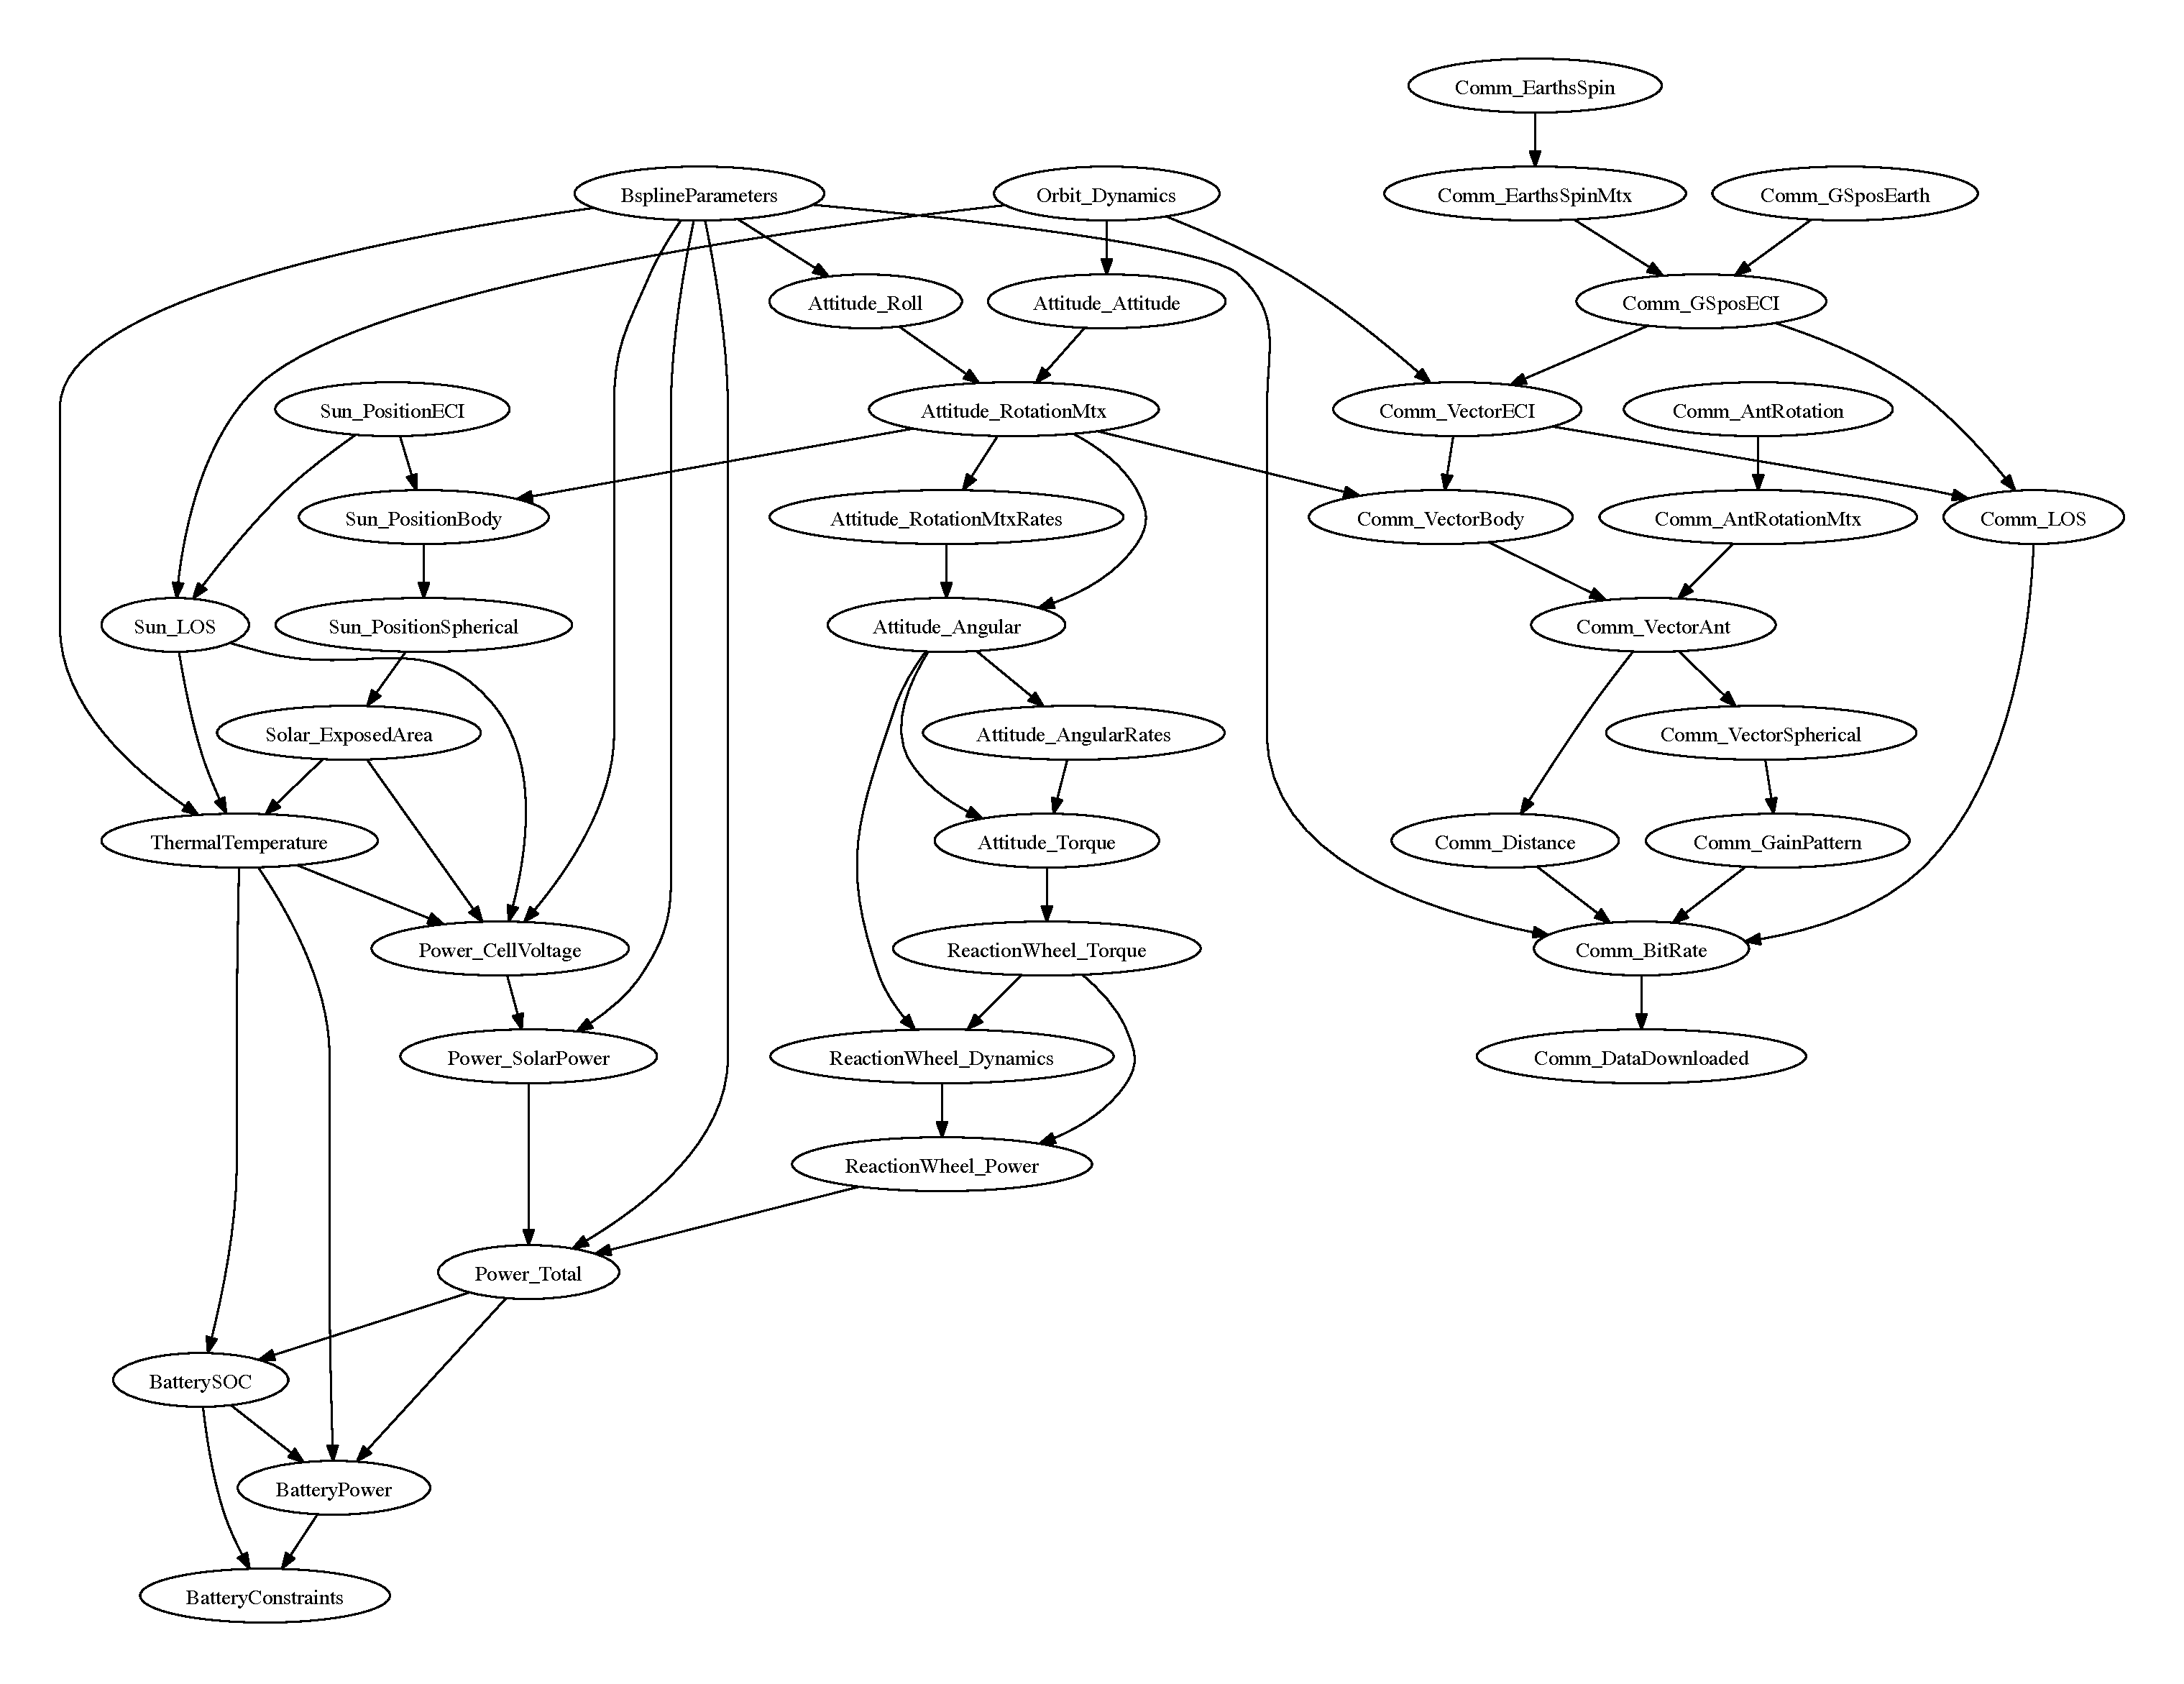
\includegraphics[width=1.1\textwidth]{images/CADRE.pdf}
          \caption{ Dependency graph for the satellite problem. \label{fig:cadre_graph}}
        \end{center}\end{figure}

        [Insert XDSM HERE]

        \begin{itemize}
            \item this problem uses adjoint
            \item all analytic gradients
        \end{itemize}


    \subsection{Results}

        \subsection{Optimization Results}

        The OpenMDAO implementation of the satellite problem was executed on a
        Macbook Pro (2.3 Ghz Core i7 processor, 4GB 1600 Mhz DDR3 memory, running OSX 10.8.5)
        over the course of two days, to a termination tolerance of $10^{-5}$. This tolerance
        was achieved within approximately 106 iterations, using the SNOPT\cite{gill2005snopt}
        optimizer.

        \begin{figure}
        \centering
        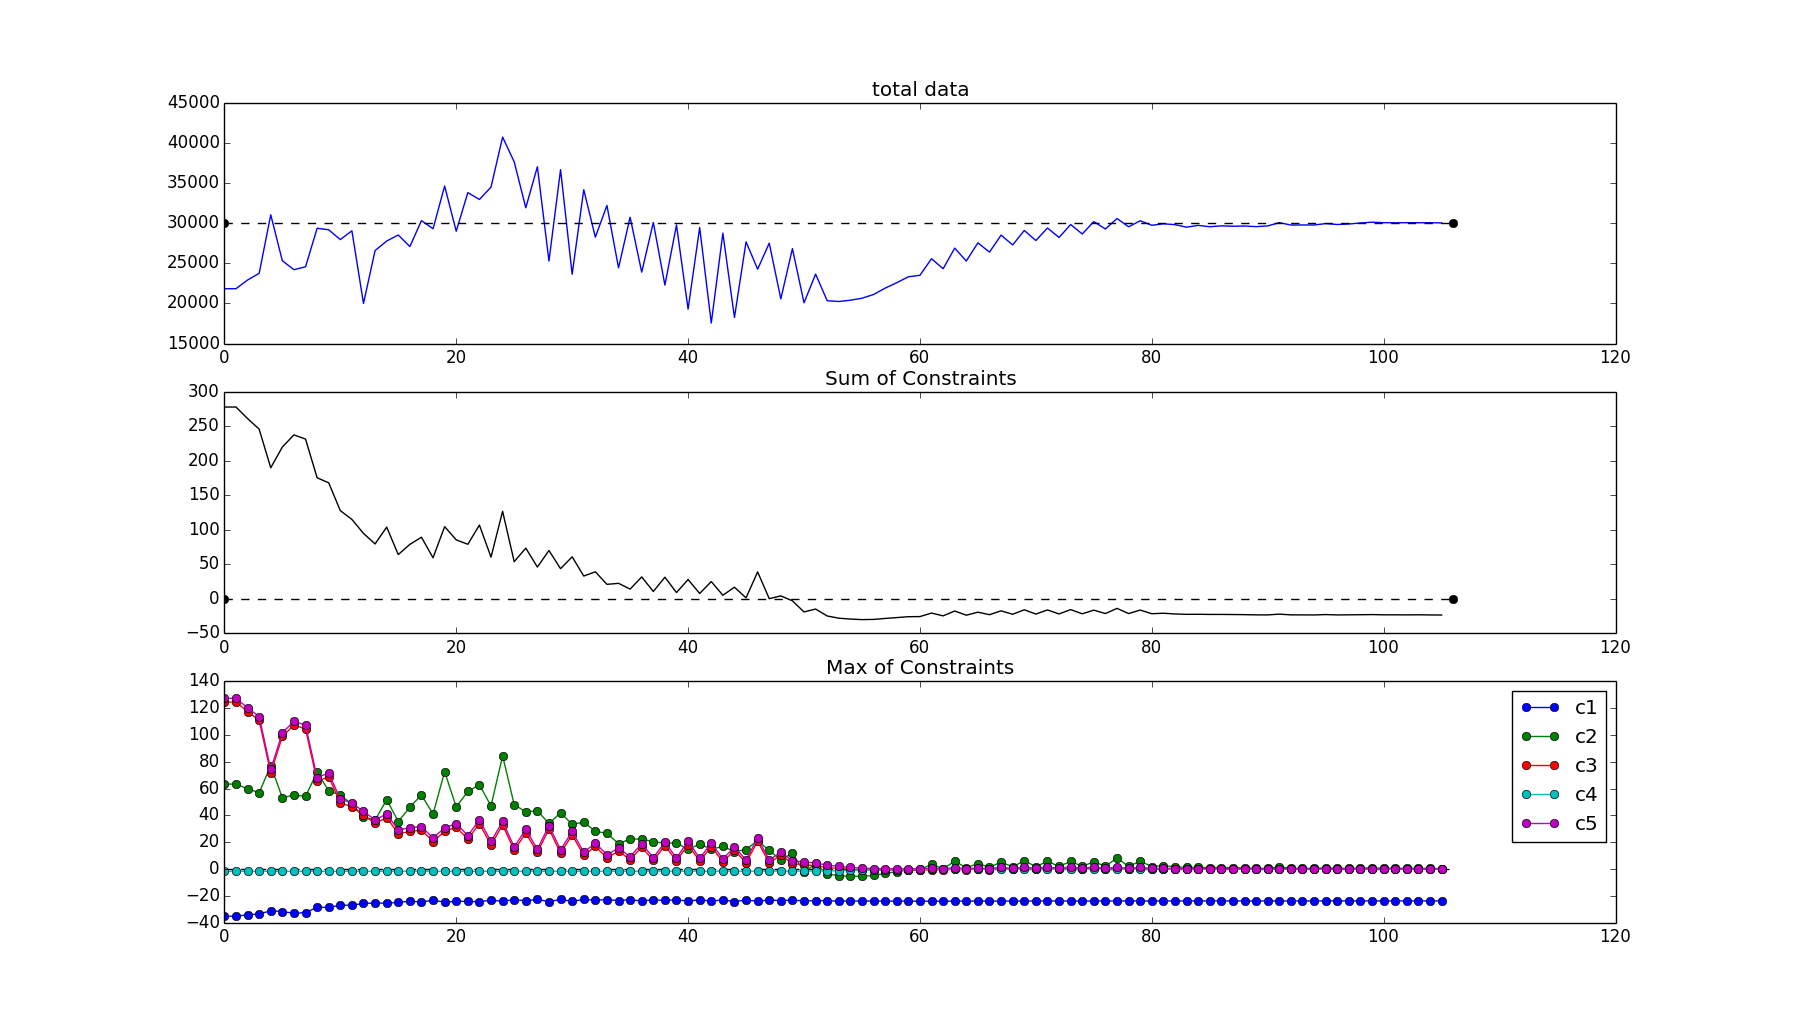
\includegraphics[width=0.99\textwidth]{images/opt}
        \caption[width=0.22\textwidth]{Convergence of the satellite problem.
        \label{convergence}
        }
        \end{figure}


        Figure \ref{convergence} illustrates the convergence of the satellite problem over the course of
        these iterations. The first row plots the
        value of the objective function, the total data downloaded over each design point. The objective
        function oscillated greatly over the course of the first half of the computed iterations, but
        stabilized by the 80th iteration near the value previously determined \cite{CADRE2012}
        to be the optimal design.

        The second row plots the maximum value of each constraint across all design points at
        each iteration. As all of the problem constraint are non-positive for a feasible design,
        this can be taken as a cursory measure of overall problem feasibility.
        The third row plots the maximum value of each constraint across each of the design points,
        but separated according to specific constraint type. These two plots both indicate that the
        oscillatory behavior of the objective function coincided with a steady decrease in design
        infeasibility. Once a feasible state was reached (near the 50th iteration), the optimizer
        began refining the design towards a more favorable value of the objective function.

        \begin{figure}
        \centering
        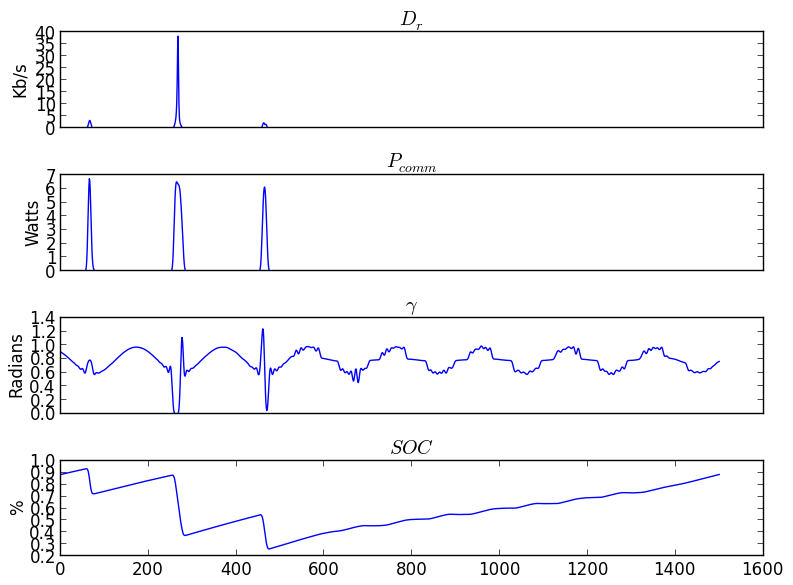
\includegraphics[width=0.8\textwidth]{images/pt_3_data}
        \caption[width=0.4\textwidth]{Plots of the bit rate, communications systems power, craft roll angle,
        and battery charge level over the half-day time period covered by the $4^{\textrm{th}}$ design point.
        \label{pt3_data_results}
        }
        \end{figure}

        Figure \ref{pt3_data_results} shows plots of selected variables for the $4^{\textrm{th}}$ design point,
        to illustrate the fidelity of the recovered solution. These variables are the communications
        bit rate ($D_r$), communications systems power level ($P_{comm}$), craft roll angle ($\gamma$),
        and battery charge level ($SOC$). Prior to the optimization, these variables
        were each instantiated to uniform values
        (across all time points) of 0, 0, $\frac{\pi}{4}$, and 0 respectively. The optimizer, operating on
        OpenMDAO's graph formulation of the problem succeeded at converging each of these variables to the values
        shown, for each time point. Line of sight is seen to have been achieved in three short ranges of time near the
        beginning of the modeled half-day design point. Interestingly, though the data rate achieved in the second
        time period with affirmative line of sight is significantly higher than the other two periods, the optimizer
        converged to a solution that provided power to the communications system near uniformly for each of these
        three time periods. This is likely due to the battery discharge rate and SOC constraints limiting
        the power which may be delivered to the communications system.

        Figure \ref{pt3_data_results} shows that the craft roll angle, $\gamma$, roughly approximates a sine function
        with a wavelength of 90 minutes (the approximate orbital period of the satellite),
        with short term perturbations during the time
        periods where line of sight is gained with the ground station. That is, the optimizer successfully
        converged to a solution with the satellite continuously turned to maximize exposure to the sun,
        except when turning to point its antenna towards the ground station during times when
        communication is possible. This dynamic is also reflected in the battery state of charge ($SOC$)
        data plotting in the bottom row, with the battery losing charge quickly during
        communication with the ground station, but recharging while tracking with the sun.

        Further post processing of the data included automatic geographical rendering of the trajectories of
        the  satellite for each of the 6 design points, using the Google
        Maps\footnote{http://developers.google.com/maps/} and Google
        Earth\footnote{http://developers.google.com/earth/} APIs. The trajectories are
        represented as polygonal chain ("polyline") elements, colored according to the
        satellites communication bit rate with the ground station during the corresponding
        window of time. Each colored line segment are centered on the locations
        determined by the time points when the data bit rate values were calculated
        by the OpenMDAO model.

        Figure \ref{pt3_g_earth} shows the communications bit rate along the trajectories of the
        satellite during the $4^{\textrm{th}}$ design point. This can be compared
        directly with Figure \ref{pt3_data_results}, where one large spike in communications
        bit rate was preceded and then succeeded by two short time periods of lesser
        data rates. Plotted geographically, this is seen to be due to the procession of
        the satellites orbit, where the period of maximal data rate corresponds to a
        pass of the satellite directly over the ground station location. The proceeding and
        succeeding data rate spikes correspond to passes over the near Atlantic and
        Rocky Mountain regions, respectively.


        Figure \ref{allpt_flatmap} similarly shows trajectory and bit rate data plotted
        from all six design points, centered on the United States. The orbital passes
        that are close enough to the ground station for communications can all be seen.
        Figure \ref{allpt_g_earth} zooms this view out to show coverage of the trajectories
        of all design points across the Earth.


        \begin{figure}
        \centering
        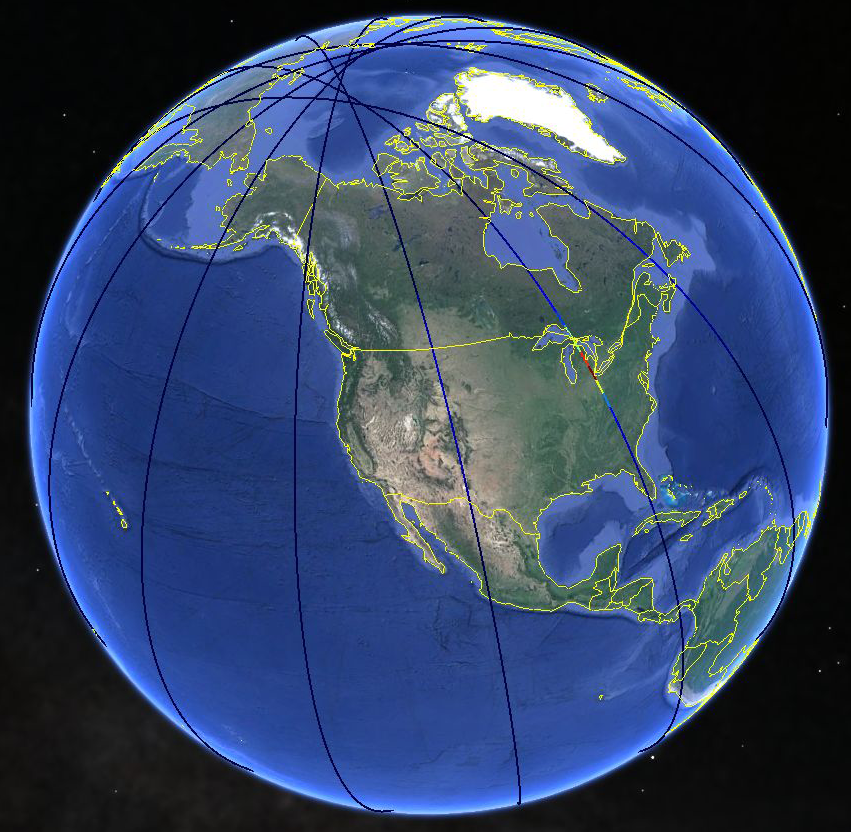
\includegraphics[width=0.8\textwidth]{images/pt3_gearth3}
        \caption[width=0.4\textwidth]{Plot of the trajectories of the satellite
        for the $4^{\textrm{th}}$ design point onto the surface of the Earth, illustrating the
        communication data rates near the ground station.
        \label{pt3_g_earth}
        }
        
        \end{figure}


        \begin{figure}
        \centering
        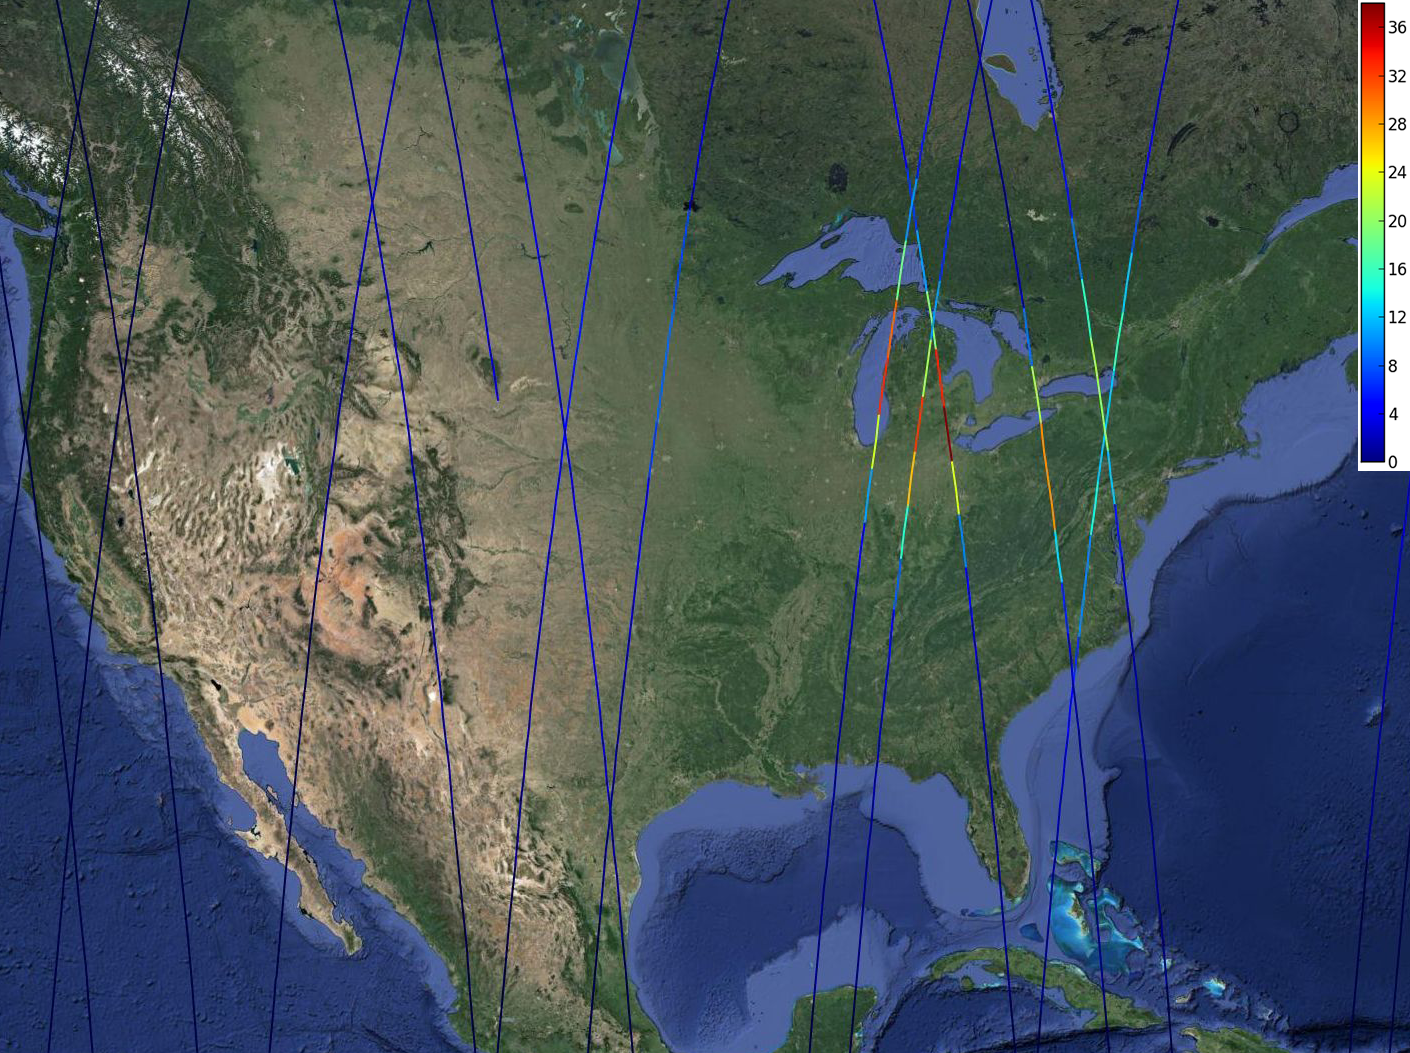
\includegraphics[width=0.8\textwidth]{images/allpts_map_data}
        \caption[width=0.4\textwidth]{Plot of the trajectories of the satellite
        for all 6 design points onto the surface of the Earth, illustrating the
        communication data rates near the ground station.
        \label{allpt_flatmap}
        }
        
        \end{figure}


        \begin{figure}
        \centering
        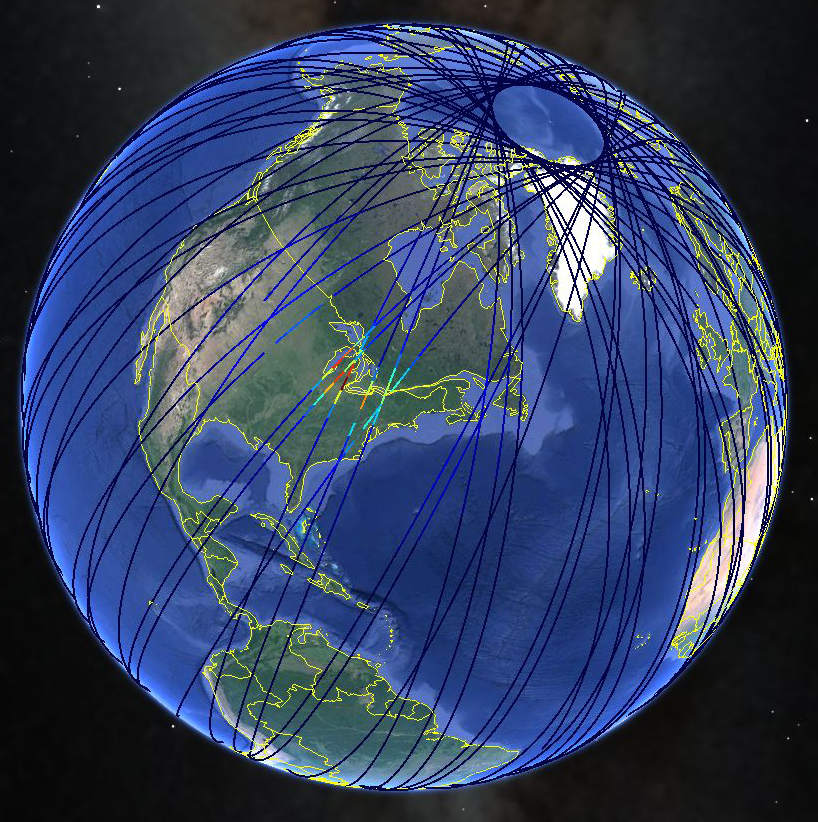
\includegraphics[width=0.8\textwidth]{images/allpts_gearth2}
        \caption[width=0.4\textwidth]{Plot of the trajectories of the satellite
        for all 6 design points onto the surface of the Earth.
        \label{allpt_g_earth}
        }
        
        \end{figure}

        \subsection{Performance Results}
            Compare size of linear system with and without sparsity. Relative speeds. 


  \section{Wind Turbine Design Problem (Justin/Andrew)}
    \subsection{Problem Formulation}
        \begin{itemize}
            \item Design variables, objectives, constraints. 
            \item this problem uses forward
            \item mixed analytic and FD gradients
            \item non-relevant, but non-differentiable variables 
        \end{itemize}

    \subsection{Results}
        \begin{itemize}
            \item FD vs analytic results
            \item speed issues without directional derivatives
        \end{itemize}
     

  \section{Conclusion (Justin/Tristan)}

      This work demonstrates how a graph-based approach to problem formulation compliments and enhances the benefits of gradient based
      optimization. The graph provides a proper structure to handle the necessary bookkeeping to automatically implement complex 
      problem formulations while making use of analytic gradients. By implementing this graph based approach in OpenMDAO, the framework 
      can alleviate the responsibilities for such bookkeeping from the user entirely which dramatically simplifies implementation. 

      The two problems examined in this work demonstrate that a single framework can operate efficiently and effectively on a wide range 
      of large-scale problems. 

  \bibliography{references}


\end{document}
